\begin{frame}{Utilité des caches}
	\begin{figure}[h!]
		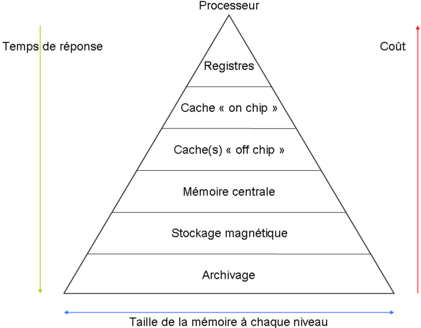
\includegraphics[scale=.6]{images/hierarchy.png}
	\end{figure}
	\begin{block}{Objectif}
		\begin{itemize}
			\item{Trouver un bon compromis entre vitesse et coût}
		\end{itemize}
	\end{block}
\end{frame}

%~ Ajouter définition de hit/miss
%~ Ajout d'une partie sur l'organisation interne d'un cache... (Set/ligne/bloc mémoire)

\begin{frame}{Associativité}
	\begin{block}{Comment localiser une donnée dans le cache ?}
		Il existe différentes fonctions de correspondance
		\begin{itemize}
			\item{Direct associative}
			\item{Fully associative}
			\item{k-ways associative}
		\end{itemize}
	\end{block}
	\begin{figure}[h!]
		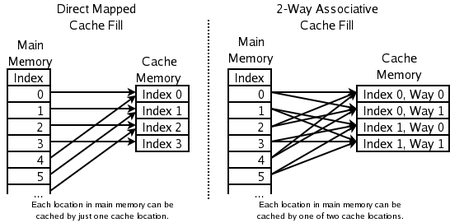
\includegraphics[scale=.4]{images/associative.png}
	\end{figure}
\end{frame}

\begin{frame}{Remplacement}
	\begin{block}{Comment ajouter une donnée dans cache plein ?}
		Il existe différentes politiques de remplacement
		\begin{itemize}
			\item{FIFO (Supprimer la plus ancienne)}
			\item{LFU (Supprimer la moins utilisée)}
			\item{LRU (Supprimer la plus anciennement utilisée)}
		\end{itemize}
	\end{block}
	Problème : Que deviennent les données évincées ?
\end{frame}

\begin{frame}{Hiérarchie de caches et problèmes de cohérence}
On utilise plusieurs niveaux de caches
%~  Schéma d'une hiérarchie de caches.
\begin{block}{Comment gérer les données entre différents niveaux?}
		\begin{itemize}
			\item{Caches inclusifs (Intel)}
			\item{Caches exclusifs (AMD)}
%~ Schéma d'illustration pour l'inclusivité ?
		\end{itemize}
	\end{block}
	\begin{block}{Comment gérer les données entre caches de même niveau?}
		Que faire lorsque deux caches doivent se partager une même donnée ?
	\end{block}
\end{frame}
